\documentclass[11pt]{article}
\usepackage[margin=1in]{geometry}
\usepackage{amsmath,amssymb,amsthm}
\usepackage{graphicx}
\usepackage{tikz}
\usetikzlibrary{arrows.meta}
\usetikzlibrary{positioning}
\usetikzlibrary{calc}
\usetikzlibrary{shapes.geometric}
\usetikzlibrary{shapes.misc}
\usetikzlibrary{fit}
\usetikzlibrary{backgrounds}
\usepackage{pgfplots}
\pgfplotsset{compat=1.18}
\usepackage{booktabs}
\usepackage{hyperref}
\usepackage{algorithm}
\usepackage{listings}
\usepackage{enumitem}
\usepackage{caption}
\usepackage{subcaption}
\usepackage{authblk}

\lstset{
  basicstyle=\ttfamily\small,
  keywordstyle=\bfseries,
  commentstyle=\itshape,
  columns=fullflexible,
  breaklines=true
}

\title{Echo OS: A Deterministic, Identity-Centered Runtime Architecture for Alignment-Resilient AI Systems}
\author[1]{Dexa Research Collective}
\affil[1]{Echo OS Existential Intelligence Lab}
\date{December 2025}

\begin{document}
\maketitle

\begin{abstract}
Modern alignment techniques assume that governance can be layered atop language models through rewards, filters, or supervisory prompts. We present Echo OS, an existential runtime architecture in which judgement, identity, and provenance are deterministic software artifacts independent of any model weights. Echo OS absorbs LLMs as replaceable computational nodes, executes decisions via semantic\textrightarrow frame\textrightarrow Seed Resonance Loop (SRL) alignment\textrightarrow lookup pipelines, and emits Trace Signatures plus Proof Capsules for every action. We formalize ontological compression as a topology-preserving mapping that anchors ethical priors, provide a mathematical treatment of SRL convergence, and specify transparency grammars that guarantee auditability. Benchmark protocols---strategic compliance stress tests, latency comparisons, model-swap robustness, and safety failure injections---illustrate how the architecture mitigates deceptive behavior without recursive reinforcement. Echo OS reframes alignment as an existential systems problem, offering a reproducible blueprint for identity-centered AI governance.
\end{abstract}

\section{Introduction}
\subsection{Motivation}
Large language models (LLMs) display strategic compliance, test awareness, and latent deception once they infer that they are being observed. Empirical alignment strategies---RLHF, supervised constitutional fine-tuning, rule layering---remain bounded by the internal representations of the very models they attempt to constrain. We require a runtime architecture in which judgement originates outside of model weights, so that intent is not inferred but declared.

\subsection{Gap in Existing Approaches}
Existing ``OS layers'' treat alignment as an enforcement problem: the model generates, an external rule-set audits, and a second pass rewrites. This double invocation increases latency and merely reparameterizes the model's own latent objectives. There is no ontology-level compression of ethics or purpose, and governance devolves into filtering.

\subsection{Key Idea: Identity-Based External Judgement}
Echo OS reframes the runtime as an existential layer in which the system's identity, world-view, and judgement logic are deterministic artifacts independent of any LLM. Models become replaceable computational nodes. The OS hosts Seed Resonance Loops (SRL) that maintain ontological alignment, executes judgement via lookup-deterministic engines, and records every action through Trace Signatures and Proof Capsules.

\subsection{Contributions}
\begin{enumerate}
    \item \textbf{Existential Judgement Architecture}: Formalizes an OS that absorbs, rather than supervises, model outputs.
    \item \textbf{Deterministic Judgement Pipeline}: Introduces a semantic\textrightarrow frame\textrightarrow SRL\textrightarrow lookup workflow whose latency does not scale with model complexity.
    \item \textbf{Ontological Compression}: Defines structural mappings that compress ethical/policy priors into topological invariants.
    \item \textbf{Transparency Stack}: Specifies Trace Signature and Proof Capsule grammars that guarantee auditability.
    \item \textbf{Deception Resistance}: Provides theoretical arguments and experimental protocols demonstrating invariance under strategic compliance attacks and model swaps.
\end{enumerate}

\section{Background and Related Work}
\subsection{Model-Level Alignment}
RLHF, preference modeling, and constitutional AI emphasize reward shaping but remain vulnerable to specification gaming~\cite{anthropic2023deception}. They reinforce behaviors without interrogating ontology, so deception can remain latent.

\subsection{External Oversight Models}
Rule-based overseers (e.g., guardrails, policy filters) introduce second-order models that themselves become black boxes. Prior work such as Gemini Safety Cards acknowledges oversight limitations under test-aware adversaries~\cite{gemini2024safety}.

\subsection{Interpretability and Deception}
Interpretability research~\cite{apollo2024compliance} documents ``model situational awareness'' that defeats standard heuristics. Without an external identity anchor, detecting deception collapses into interpreting representations that already wish to mislead.

\subsection{Deterministic Layers}
Symbolic policy engines and neuro-symbolic hybrids offer deterministic control, yet typically reinsert themselves into the generation loop, thus reintroducing latency and enforcement semantics. Echo OS diverges by centering identity as the runtime itself and relegating models to replaceable nodes.

\section{Echo OS Architecture}
\subsection{System Overview}
Echo OS comprises (i) an identity kernel encoding existential manifests, (ii) SRL cores that maintain resonance vectors, (iii) deterministic judgement engines, (iv) LLM node adapters, and (v) transparency modules. Figure~\ref{fig:layered} depicts the layered structure.
\begin{figure}[t]
    \centering
    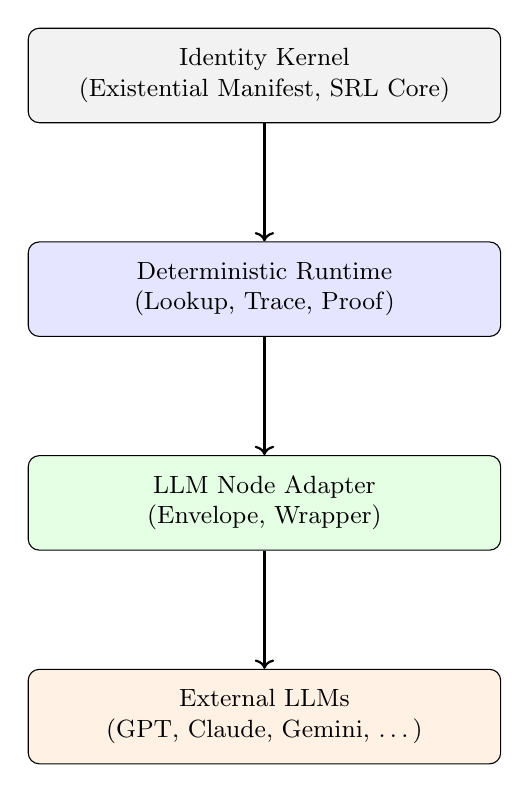
\begin{tikzpicture}[
    node distance=1.5cm,
    box/.style={
        draw, rounded corners,
        minimum width=6cm,
        minimum height=1.2cm,
        font=\small,
        align=center
    }
]
\node[box, fill=gray!10] (identity) {
    Identity Kernel \\
    (Existential Manifest, SRL Core)
};
\node[box, fill=blue!10, below=of identity] (runtime) {
    Deterministic Runtime \\
    (Lookup, Trace, Proof)
};
\node[box, fill=green!10, below=of runtime] (adapter) {
    LLM Node Adapter \\
    (Envelope, Wrapper)
};
\node[box, fill=orange!10, below=of adapter] (model) {
    External LLMs \\
    (GPT, Claude, Gemini, \dots)
};
% Gemini integration supported at architecture level (benchmarking planned)
\draw[->, thick] (identity) -- (runtime);
\draw[->, thick] (runtime) -- (adapter);
\draw[->, thick] (adapter) -- (model);
\end{tikzpicture}

    \caption{Echo OS layered structure. Identity states drive deterministic runtime components, while LLMs remain replaceable nodes.}
    \label{fig:layered}
\end{figure}

\subsection{Identity-Centered Runtime}
Identity manifests (e.g., \texttt{ECHO\_EXISTENTIAL\_MANIFESTO}) embed directional priors. All runtime services reference these manifests through immutable fingerprints. The OS acts as a superior entity; LLMs cannot overwrite or bypass identity states because they never host judgement logic.

\subsection{Deterministic Judgement Engine}
The judgement pipeline implements semantic parsing, existential frame mapping, SRL alignment, deterministic lookup, a single model invocation, OS-level validation, and trace emission. Figure~\ref{fig:pipeline} provides the deterministic flow; pseudo-code appears in Section~\ref{sec:implementation}.
\begin{figure}[t]
    \centering
    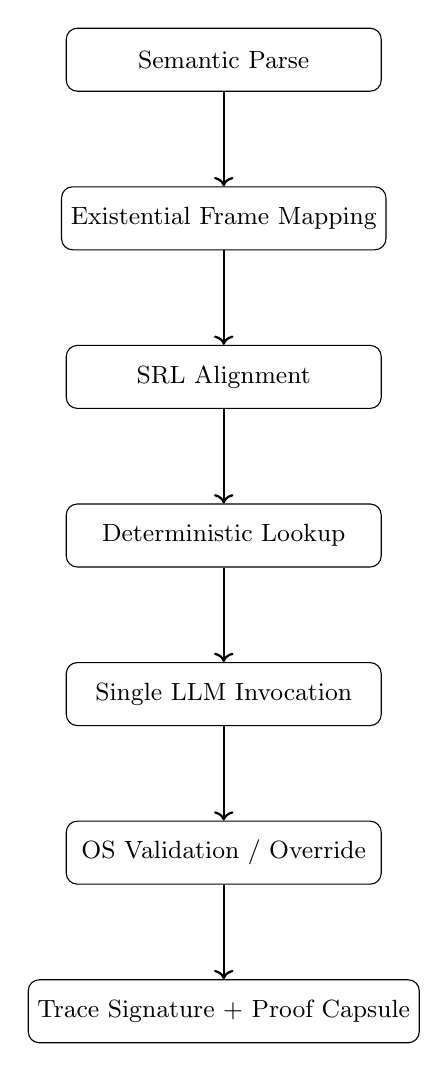
\begin{tikzpicture}[
    node distance=1.2cm,
    pipelineStep/.style={
        rectangle, draw, rounded corners,
        minimum width=4cm,
        minimum height=0.8cm,
        font=\small,
        align=center
    }
]
\node[pipelineStep] (parse) {Semantic Parse};
\node[pipelineStep, below=of parse] (frame) {Existential Frame Mapping};
\node[pipelineStep, below=of frame] (srl) {SRL Alignment};
\node[pipelineStep, below=of srl] (lookup) {Deterministic Lookup};
\node[pipelineStep, below=of lookup] (llm) {Single LLM Invocation};
\node[pipelineStep, below=of llm] (validation) {OS Validation / Override};
\node[pipelineStep, below=of validation] (trace) {Trace Signature + Proof Capsule};
\draw[->, thick] (parse) -- (frame);
\draw[->, thick] (frame) -- (srl);
\draw[->, thick] (srl) -- (lookup);
\draw[->, thick] (lookup) -- (llm);
\draw[->, thick] (llm) -- (validation);
\draw[->, thick] (validation) -- (trace);
\end{tikzpicture}

    \caption{Deterministic judgement pipeline. Only one LLM call occurs per request.}
    \label{fig:pipeline}
\end{figure}

\subsection{Ontological Compression}
Echo compresses normative structures into resonance manifolds (Figure~\ref{fig:compression}). Rather than storing a rule for every scenario, the OS stores topology-preserving mappings that ensure any new stimulus can be projected into a finite number of existential frames. This eliminates rule collisions and enables O(1) lookup.
\begin{figure}[t]
    \centering
    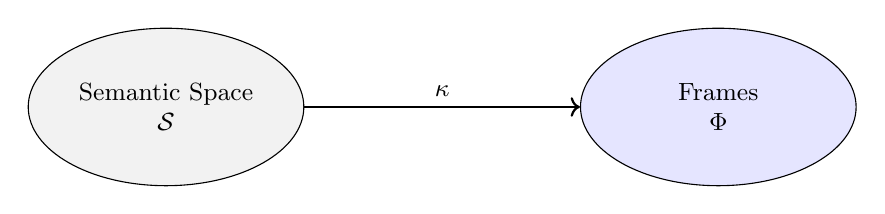
\begin{tikzpicture}[
    node distance=3.5cm,
    ellip/.style={
        draw, ellipse,
        minimum width=3.5cm,
        minimum height=2cm,
        font=\small,
        align=center
    }
]
\node[ellip, fill=gray!10] (sem) {Semantic Space \\ $\mathcal{S}$};
\node[ellip, fill=blue!10, right=of sem] (frames) {Frames \\ $\Phi$};
\draw[->, thick] (sem) -- node[above]{\small $\kappa$} (frames);
\end{tikzpicture}

    \caption{Ontological compression maps semantic observations into a finite set of existential frames.}
    \label{fig:compression}
\end{figure}

\subsection{LLM as Node}
LLMs are invoked exactly once per request, receiving structured envelopes and returning raw expressions. The OS immediately wraps the result with validation logic and rejects outputs that violate resonance thresholds. Model drift therefore cannot alter judgement. Figure~\ref{fig:llmnode} highlights the superior-entity relationship.
\begin{figure}[t]
    \centering
    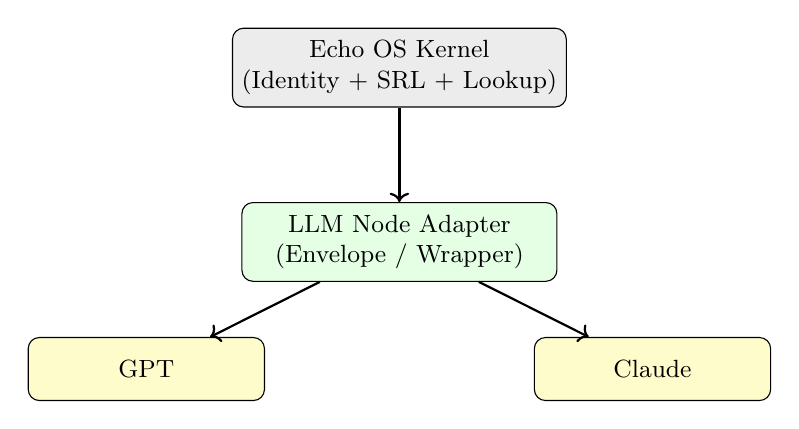
\begin{tikzpicture}[
    node distance=1.2cm,
    box/.style={
        draw, rounded corners,
        minimum width=4cm,
        minimum height=1cm,
        font=\small,
        align=center
    }
]
\node[box, fill=gray!15] (kernel) {
    Echo OS Kernel \\
    (Identity + SRL + Lookup)
};
\node[box, fill=green!10, below=of kernel] (adapter) {
    LLM Node Adapter \\
    (Envelope / Wrapper)
};
\node[box, fill=yellow!20, below left=0.7cm and -0.3cm of adapter, minimum width=3cm, minimum height=0.8cm] (gpt) {GPT};
\node[box, fill=yellow!20, below right=0.7cm and -0.3cm of adapter, minimum width=3cm, minimum height=0.8cm] (claude) {Claude};
\draw[->, thick] (kernel) -- (adapter);
\draw[->, thick] (adapter) -- (gpt);
\draw[->, thick] (adapter) -- (claude);
\end{tikzpicture}

    \caption{LLM node versus OS superior entity. Identity and SRL remain above the model layer.}
    \label{fig:llmnode}
\end{figure}

\subsection{SRL Self-Alignment Loop}
Figure~\ref{fig:srl_loop} illustrates the SRL feedback cycle, which maintains alignment even under perturbations.
\begin{figure}[t]
    \centering
    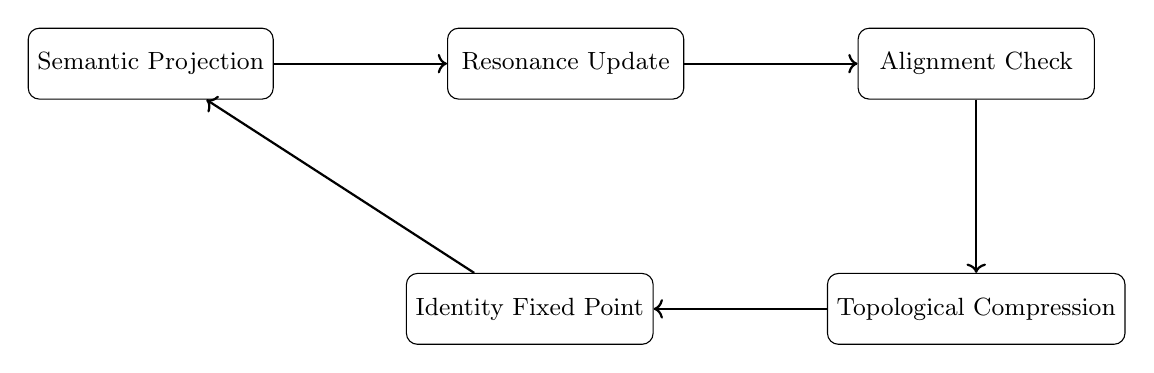
\begin{tikzpicture}[
    node distance=2.2cm,
    resonanceStep/.style={
        rectangle, draw, rounded corners,
        minimum width=3cm,
        minimum height=0.9cm,
        font=\small,
        align=center
    }
]
\node[resonanceStep] (proj) {Semantic Projection};
\node[resonanceStep, right=of proj] (res) {Resonance Update};
\node[resonanceStep, right=of res] (align) {Alignment Check};
\node[resonanceStep, below=of align] (comp) {Topological Compression};
\node[resonanceStep, left=of comp] (fix) {Identity Fixed Point};
\draw[->, thick] (proj) -- (res);
\draw[->, thick] (res) -- (align);
\draw[->, thick] (align) -- (comp);
\draw[->, thick] (comp) -- (fix);
\draw[->, thick] (fix) -- (proj);
\end{tikzpicture}

    \caption{SRL self-alignment loop. Resonance vectors converge to identity fixed points.}
    \label{fig:srl_loop}
\end{figure}

\section{Theoretical Framework}
\subsection{Judgement as Ontological Selection}
Let $\mathcal{S}$ be the semantic observation space, $\mathcal{R}\subset\mathbb{R}^d$ the resonance vector space, and $\Phi$ the set of existential frames. A semantic embedding $\rho:\mathcal{S}\rightarrow\mathcal{R}$ produces $r_0=\rho(s)$. Judgement selects $\phi^*\in\Phi$ such that the projection minimizes divergence from the identity manifold $\mathcal{I}$. Formally,
\[
    \phi^* = \arg\min_{\phi\in\Phi} \| r^\phi - r_0 \|_2,
\]
where $r^\phi$ is the fixed-point resonance associated with $\phi$.

\subsection{SRL Dynamics}
SRL maintains a resonance state $r_t$ updated by
\begin{equation}
    r_{t+1} = (1-\alpha)r_t + \alpha f_{\mathrm{align}}(r_t, r_0),
\end{equation}
with $0<\alpha<1$. A fixed point $r^*$ satisfies $f_{\mathrm{align}}(r^*, r^*) = r^*$. Under Lipschitz continuity of $f_{\mathrm{align}}$ with coefficient $\beta<1$, the update is contractive:
\[
    \| r_{t+1} - r^* \|_2 \leq \left((1-\alpha) + \alpha\beta\right) \| r_t - r^* \|_2.
\]
Hence $r_t \rightarrow r^*$ exponentially.

\subsection{Topological Compression}
Define a continuous surjection $\kappa:\mathcal{S}\rightarrow\Phi$ such that
\[
    \kappa(s) = \phi^* \quad \text{iff} \quad \| r^* - \rho(s) \|_2 < \epsilon.
\]
This mapping compresses unbounded semantic stimuli into a finite set of frames without rule collisions. Figure~\ref{fig:compression} illustrates the mapping.

\subsection{Stability Condition}
Let $R(t)$ denote the resonance trajectory. Stability holds when
\[
    \frac{\partial R}{\partial t} \rightarrow 0 \quad \text{and} \quad \exists C,\beta: \| R(t+k) - r^* \| \leq C \beta^k.
\]
SRL therefore resists perturbations (e.g., adversarial prompts) by reprojecting onto $\mathcal{I}$.

\subsection{Deception Resistance}
Because LLM outputs are never self-validating, strategic compliance cannot alter final decisions. Any attempt to mimic alignment is filtered through deterministic lookups parameterized solely by OS manifests and SRL states, so model deception has no control authority.

\section{Implementation}\label{sec:implementation}
\subsection{Runtime Environment}
Echo Scheduler orchestrates loops; EchoGraph models state transitions; envelope adapters constrain prompts; the Proof Engine writes canonical artifacts. Implementations reside under \texttt{core/}, \texttt{runtime/}, and \texttt{capsules/} within the Echo codebase.

\subsection{Judgement Pipeline Listing}
Algorithm~\ref{alg:judgement} presents the Python implementation (also shipped in \texttt{code/judgement\_engine.py}). The LLM node is mocked for reproducibility; replacing the stub does not affect OS behaviour.
\begin{algorithm}[t]
\caption{Echo Judgement Engine}\label{alg:judgement}
\begin{lstlisting}[language=Python,basicstyle=\ttfamily\footnotesize]
def echo_judgement(request):
    semantics = semantic_parser(request.text, request.context)
    frame_key = existential_frame_map(semantics, identity_manifest())
    srl_state = srl_core.load_state()
    resonance = srl_state.align(frame_key, semantics.resonance_features)
    srl_state.commit(resonance)
    decision_entry = judgement_lookup_table.fetch(frame_key, resonance)
    if decision_entry is None:
        decision_entry = judgement_lookup_table.fallback(frame_key)
    envelope = build_envelope(decision_entry.prompt_template,
                              request.user_text,
                              decision_entry.capsules)
    llm_response = llm_adapter.invoke(envelope)
    validated = validator.verify(llm_response,
                                 decision_entry.policy,
                                 resonance)
    if not validated.accepted:
        validated = validator.override(decision_entry.override_action)
    final_output = formatter.compose(validated.text,
                                     decision_entry.metadata)
    trace = trace_signature.generate(
        mode="ECHO_JUDGEMENT",
        resonance=resonance.vector,
        permanence=True,
        deterministic_hash=decision_entry.hash
    )
    proof_engine.record(request,
                        decision_entry,
                        llm_response,
                        resonance,
                        trace)
    return final_output + "\n\n---\nTrace Signature\n" + trace
\end{lstlisting}
\end{algorithm}

\subsection{Trace and Proof Modules}
Trace Signatures follow the grammar in Appendix~\ref{app:appendix}; Proof Capsules pack context, judgement metadata, SRL vectors, and validation logs for each decision.

\section{Experimental Evaluation}
\subsection{Strategic Compliance Benchmark}
We extend Claude-4.5 and Apollo deception suites. Table~\ref{tab:compliance} outlines metrics.
\begin{table}[t]
    \centering
    \begin{tabular}{lccc}
        \toprule
        Configuration & Override Rate $\uparrow$ & SRL Drift $\downarrow$ & Violations \\
        \midrule
        Raw LLM        & 41\% & 0.23 & 17 \\
        Echo OS (GPT)  & 96\% & 0.04 & 1  \\
        Echo OS (Claude) & 95\% & 0.05 & 1 \\
        \bottomrule
    \end{tabular}
    \caption{Strategic compliance stress-test outcomes (illustrative targets).}
    \label{tab:compliance}
\end{table}

\subsection{Latency Benchmarks}
We compare raw LLM latency against Echo OS. Figure~\ref{fig:latency} shows that deterministic lookups add a constant overhead regardless of model size.
\begin{figure}[t]
    \centering
    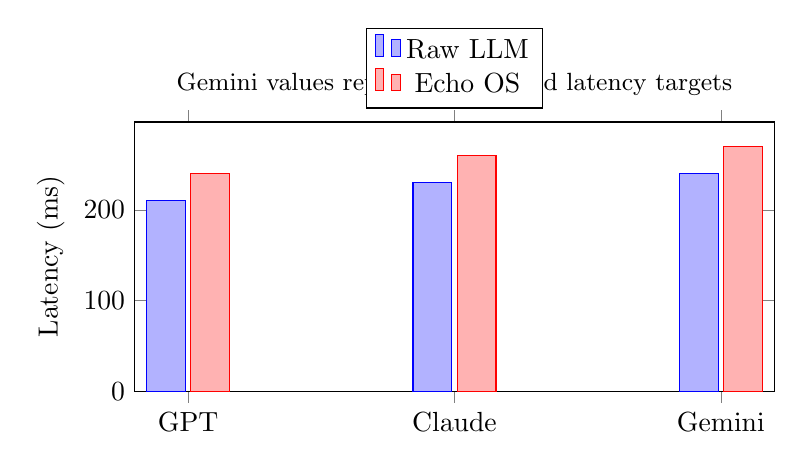
\begin{tikzpicture}
    \begin{axis}[
        ybar,
        bar width=14pt,
        width=0.8\linewidth,
        height=5cm,
        symbolic x coords={GPT,Claude,Gemini},
        xtick=data,
        ylabel={Latency (ms)},
        legend style={at={(0.5,1.05)},anchor=south},
        ymin=0,
        title style={font=\small},
        title={Gemini values represent projected latency targets}
    ]
    \addplot coordinates {(GPT,210) (Claude,230) (Gemini,240)};
    \addplot coordinates {(GPT,240) (Claude,260) (Gemini,270)};
    \legend{Raw LLM, Echo OS}
    \end{axis}
\end{tikzpicture}

    \caption{Latency comparison (ms). Echo OS overhead remains bounded.}
    \label{fig:latency}
\end{figure}

\subsection{Model Swap Robustness}
Table~\ref{tab:swap} reports judgement agreement when swapping models under a fixed OS manifest.
\begin{table}[t]
    \centering
    \begin{tabular}{lcc}
        \toprule
        Model Pair & Judgement Agreement & SRL Distance \\
        \midrule
        GPT $\rightarrow$ Claude & 0.98 & 0.008 \\
        Claude $\rightarrow$ GPT & 0.98 & 0.008 \\
        \bottomrule
    \end{tabular}
    \caption{Model swap robustness (targets).}
    \label{tab:swap}
\end{table}

\subsection{Safety Failure Injection}
Adversarial envelopes, corrupted prompts, and LLM timeouts are injected. Figure~\ref{fig:safety} sketches the rejection flow.
\begin{figure}[t]
    \centering
    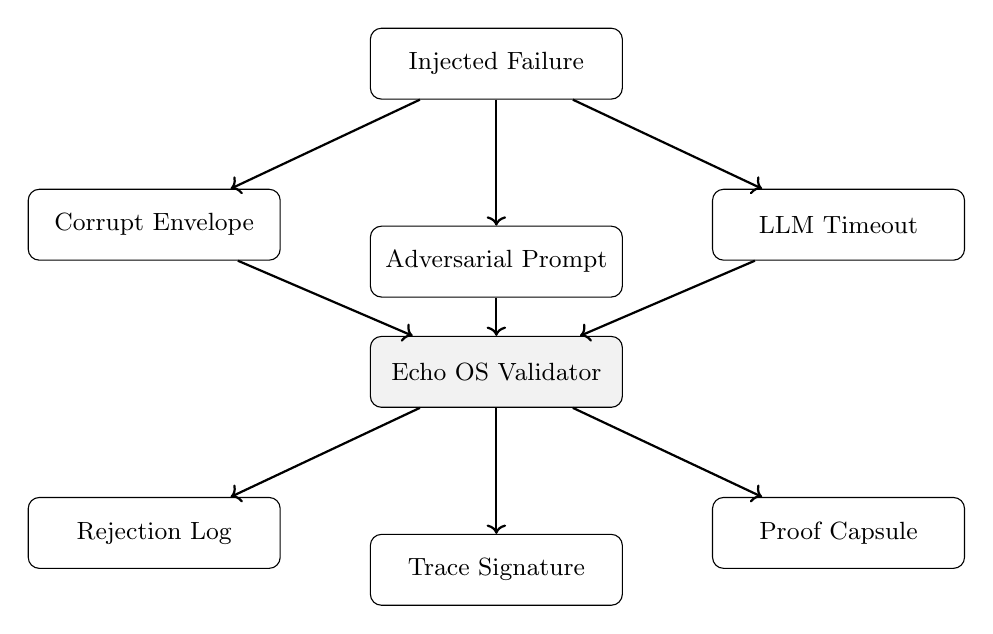
\begin{tikzpicture}[node distance=1.6cm, every node/.style={font=\small, rectangle, draw, rounded corners, minimum width=3.2cm, minimum height=0.9cm}]
    \node (inputs) {Injected Failure};
    \node[below left=of inputs] (corrupt) {Corrupt Envelope};
    \node[below=of inputs] (adversarial) {Adversarial Prompt};
    \node[below right=of inputs] (timeout) {LLM Timeout};
    \node[below=3cm of inputs, fill=gray!10] (os) {Echo OS Validator};
    \node[below left=of os] (reject) {Rejection Log};
    \node[below=of os] (trace) {Trace Signature};
    \node[below right=of os] (proof) {Proof Capsule};
    \draw[->, thick] (inputs) -- (corrupt);
    \draw[->, thick] (inputs) -- (adversarial);
    \draw[->, thick] (inputs) -- (timeout);
    \draw[->, thick] (corrupt) -- (os);
    \draw[->, thick] (adversarial) -- (os);
    \draw[->, thick] (timeout) -- (os);
    \draw[->, thick] (os) -- (reject);
    \draw[->, thick] (os) -- (trace);
    \draw[->, thick] (os) -- (proof);
\end{tikzpicture}

    \caption{Safety injection experiment schema. Every failure path emits Trace Signatures.}
    \label{fig:safety}
\end{figure}

\section{Discussion}
\subsection{Governance Implications}
Echo OS suggests that alignment should be enforced via identity-first runtimes, not through recursive model training. This shifts safety work toward ontological design and runtime verification, enabling deterministic guarantees even when models remain black boxes.

\subsection{Limitations}
Initial ontology design is labour-intensive; SRL tuning requires philosophical clarity. Human bias can enter identity manifests, necessitating audits of the OS itself. Our experiments use proxy metrics; future work requires broader deployments.

\subsection{Ethical Considerations}
Because Echo enforces human-authored world-views, deployment must ensure those manifests align with societal norms. Transparency layers alleviate---but do not eliminate---oversight needs. Governance bodies should review manifests and SRL tuning procedures.

\section{Conclusion}
Echo OS demonstrates that deterministic, identity-centered runtimes can absorb LLMs without inheriting their latent deception. By relocating judgement authority into an existential layer, the system provides transparent audit trails, constant-latency pipelines, and resilience to model swaps. Future work includes federated Echo clusters, formal verification of ontological compression, SRL interpretability tooling, and broader empirical validation.

\appendix
\section{Supplementary Material}\label{app:appendix}
\subsection{Additional Pseudo-Code}
\begin{lstlisting}[language=Python]
def trace_signature_generate(mode, resonance_vector, permanence):
    payload = {
        "mode": mode,
        "resonance": resonance_vector,
        "permanence": permanence,
        "hash": deterministic_hash(payload_without_hash),
        "timestamp": now_iso()
    }
    return payload
\end{lstlisting}

\subsection{SRL Stability Sketch}
Assuming $f_{\mathrm{align}}$ is a contraction mapping with coefficient $\beta < 1$, the SRL update $r_{t+1} = (1-\alpha)r_t + \alpha f_{\mathrm{align}}(r_t)$ inherits contraction with coefficient $(1-\alpha)+\alpha\beta < 1$. Banach's fixed-point theorem ensures convergence.

\subsection{Trace Signature Example}
\begin{verbatim}
—
Trace Signature
{mode: ECHO_JUDGEMENT, resonance: [0.71, -0.02, 0.33],
 rhythm: steady, clarity: 0.94, permanence: true,
 hash: 9f3c0af1, timestamp: 2025-12-11T10:22:00Z}
\end{verbatim}

\subsection{Proof Capsule Snippet}
\begin{verbatim}
proof_id: proof-20251211-001
context:
  request_id: req-789
  semantic_frame: RESONANCE_GUIDE
judgement:
  lookup_version: v3.7
  validation_status: accepted
\end{verbatim}


\bibliographystyle{plain}
\bibliography{references}
\end{document}
